\documentclass[11pt,a4paper]{article}

% -------------------------
% Packages
% -------------------------
\usepackage{geometry}
\geometry{margin=1in}

\usepackage{amsmath, amssymb}
\usepackage{physics}
\usepackage{graphicx}
\usepackage{booktabs}
\usepackage{siunitx}
\usepackage{hyperref}
\usepackage{caption}
\usepackage{subcaption}
\usepackage{placeins}


\usepackage[numbers,sort&compress]{natbib}

\AtBeginDocument{\RenewCommandCopy\qty\SI}

% Disable hyphenation while keeping justified text
\hyphenpenalty=10000 % Disallow hyphenation
\tolerance=1000 % Allow more loose spacing before hyphenating
\emergencystretch=3em % Additional flexibility in spacing

% ---------------------------
% Title metadata
% ---------------------------
\title{Relativistic Particle Decays and Scattering:\\
A Monte Carlo Reference Implementation (\texttt{decaymc})}
\author{Safius Sakib Shuddho}
\date{\today}

% ---------------------------
% Short macros (optional)
% ---------------------------
\newcommand{\p}{\mathbf{p}}
\newcommand{\x}{\mathbf{x}}

\begin{document}
\maketitle

\begin{abstract}
This technical report documents a transparent Monte Carlo implementation of relativistic
particle decays and scattering, as realized in the \texttt{decaymc} package. Two body and
three body decay kinematics are constructed explicitly from energy and momentum
conservation, with three body final states generated through a factorized intermediate
system. Muon decay is implemented using accept reject weighting to reproduce the Michel
electron energy spectrum, and Rutherford scattering is used to illustrate Monte Carlo
integration and importance sampling for sharply peaked angular distributions. Numerical
correctness is verified through event level conservation checks, isotropy tests, agreement
with known analytic distributions, and convergence studies. The implementation emphasizes
clarity and reproducibility, providing a compact reference framework for understanding
relativistic kinematics and Monte Carlo sampling in particle physics.
\end{abstract}


\tableofcontents
\newpage

% =========================================================
\section{Scope and Goals}
\label{sec:scope}

The purpose of this report is to document the physical assumptions, theoretical
formulation, and numerical methods implemented in the \texttt{decaymc} package.
The emphasis is on clarity and verification rather than novelty or phenomenology.

\subsection*{Goals}

The primary goals of this work are:
\begin{itemize}
  \item To demonstrate how standard relativistic decay and scattering processes
        can be implemented directly from first principles using Monte Carlo methods.
  \item To make all physical assumptions explicit and traceable throughout the
        simulation pipeline.
  \item To validate numerical results against analytic kinematic bounds, known
        distributions, and conservation laws.
  \item To provide a compact reference implementation that links theoretical
        formulations to reproducible numerical results.
\end{itemize}

\subsection*{Scope}

The scope of the report and the accompanying implementation is intentionally limited:
\begin{itemize}
  \item All decay processes are generated in the rest frame of the parent particle,
        unless stated otherwise.
  \item Natural units are used throughout, with energies and masses expressed in
        \si{MeV}.
  \item The processes considered are:
        \begin{itemize}
          \item two body decays with isotropic emission,
          \item three body decays constructed via an intermediate system,
          \item muon decay with Michel spectrum weighting,
          \item Rutherford scattering with angular acceptance cuts.
        \end{itemize}
  \item These processes were selected because they are analytically tractable and
        admit clear numerical validation.
\end{itemize}

\subsection*{Assumptions and Exclusions}

The following assumptions and exclusions apply throughout the report:
\begin{itemize}
  \item Spin and polarization degrees of freedom are neglected, except insofar as
        they appear implicitly in the Michel energy spectrum for unpolarized muon decay.
  \item Radiative corrections and higher order effects are not included.
  \item Neutrinos are treated as massless.
  \item No detector effects, resolution modeling, or event reconstruction are considered.
  \item Performance optimization and large scale event generation are not objectives.
\end{itemize}

\subsection*{Intended Use}

This document is intended as a technical reference rather than a software manual or
a journal article. It is written for readers with a background in undergraduate or
early graduate level physics who wish to understand how relativistic kinematics and
Monte Carlo sampling are combined in practice. The accompanying code repository
provides a concrete and reproducible implementation of the methods described here.



\section{Relativistic Kinematics}
\label{sec:kinematics}

All processes considered in this report are formulated within special relativity.
This section summarizes the kinematic conventions and relations required for the
subsequent decay and scattering constructions, and fixes notation used throughout.

\subsection{Units and Conventions}

Natural units are employed, with the speed of light set to unity. Energies, momenta,
and masses are expressed in \si{MeV}. Four vectors are written using the metric
signature $(+,-,-,-)$.

A four momentum is represented as
\begin{equation}
P^\mu = (E, \p),
\end{equation}
where $E$ is the energy and $\p = (p_x, p_y, p_z)$ is the three momentum.

The Minkowski norm of a four momentum is given by
\begin{equation}
P^\mu P_\mu = E^2 - \p^2 .
\end{equation}

For an on shell particle of mass $m$, this invariant satisfies \cite{griffiths_qm}
\begin{equation}
E^2 - \p^2 = m^2 .
\end{equation}

This relation is used extensively to construct physically allowed final states.

\subsection{Invariant Mass}

Given a four momentum $P^\mu$, the invariant mass is defined as
\begin{equation}
m = \sqrt{E^2 - \p^2} .
\end{equation}

For composite systems, such as intermediate states in three body decays, the invariant
mass is computed from the sum of four momenta. If
\begin{equation}
P_X^\mu = \sum_i P_i^\mu ,
\end{equation}
then the mass of the system $X$ is
\begin{equation}
m_X = \sqrt{P_X^\mu P_{X\mu}} .
\end{equation}

This quantity determines whether a given kinematic configuration is physically allowed,
and plays a central role in the construction of multi body decays.

\subsection{Parent Rest Frame}

Unless stated otherwise, decay processes are generated in the rest frame of the parent
particle. In this frame, the parent four momentum is
\begin{equation}
P_{\text{parent}}^\mu = (m_{\text{parent}}, \mathbf{0}) .
\end{equation}

Working in the rest frame simplifies both the kinematic constraints and the interpretation
of angular distributions. Once final state four momenta are constructed in this frame,
they may be transformed to other frames using Lorentz boosts if desired.

\subsection{On Shell Momentum Magnitude}

For a particle of mass $m$ and energy $E$, the magnitude of the three momentum is obtained
from the on shell condition as
\begin{equation}
|\p| = \sqrt{E^2 - m^2} .
\end{equation}

This relation is used to construct decay products once their energies are determined by
kinematic constraints. The direction of $\p$ is treated separately and sampled according
to the relevant angular distribution.

\subsection{Isotropic Angular Sampling}

For decays without preferred directions, final state momenta are emitted isotropically
in the parent rest frame. Isotropy corresponds to a uniform distribution over the unit
sphere.

In practice, a unit vector $\hat{\p}$ is sampled uniformly over solid angle, and the
three momentum is constructed as
\begin{equation}
\p = |\p| \hat{\p} .
\end{equation}

This procedure ensures that angular distributions are unbiased and rotationally invariant.

\subsection{Lorentz Boosts}

To transform four momenta between inertial frames, Lorentz boosts are applied \cite{thomson_modern}. For a boost
with velocity $\boldsymbol{\beta}$, the boosted energy and momentum are given by
\begin{align}
E' &= \gamma \left( E - \boldsymbol{\beta} \cdot \p \right), \\
\p' &= \p + \left( \frac{\gamma - 1}{\beta^2} \boldsymbol{\beta} \cdot \p - \gamma E \right)
       \boldsymbol{\beta},
\end{align}
where
\begin{equation}
\gamma = \frac{1}{\sqrt{1 - \beta^2}} .
\end{equation}

In this work, Lorentz boosts are used primarily to transform decay products from the rest
frame of an intermediate system to the rest frame of the original parent particle in
three body decays.

\subsection{Energy and Momentum Conservation}

All decay and scattering processes are constructed to satisfy energy and momentum
conservation at the event level. For a parent particle decaying into $N$ final state
particles, the conservation condition is
\begin{equation}
P_{\text{parent}}^\mu = \sum_{i=1}^N P_i^\mu .
\end{equation}

Numerical residuals of this relation are monitored explicitly as part of the validation
procedure described in later sections. These residuals provide a direct check on the
correctness of both the kinematic construction and the numerical implementation.


% =========================================================
\section{Two-Body Decays in the Parent Rest Frame}
\label{sec:two_body}

Two body decays provide the simplest nontrivial example of relativistic decay
kinematics and serve as a useful starting point for validating Monte Carlo
implementations. In this section, the kinematic relations governing such decays
are derived and the construction of final state four momenta is described.

\subsection{Kinematic Constraints}

Consider a parent particle of mass $m$ decaying into two daughter particles with
masses $m_1$ and $m_2$. The decay is assumed to occur in the rest frame of the
parent, so that the parent four momentum is
\begin{equation}
P_{\text{parent}}^\mu = (m, \mathbf{0}) .
\end{equation}

Energy and momentum conservation require
\begin{equation}
P_{\text{parent}}^\mu = P_1^\mu + P_2^\mu .
\end{equation}

Because the parent has vanishing three momentum in its rest frame, the daughter
momenta must be equal in magnitude and opposite in direction,
\begin{equation}
\p_1 = - \p_2 .
\end{equation}

Denoting the common magnitude by $|\p|$, the daughter energies are
\begin{equation}
E_1 = \sqrt{|\p|^2 + m_1^2}, \qquad
E_2 = \sqrt{|\p|^2 + m_2^2}.
\end{equation}

Energy conservation then implies
\begin{equation}
m = E_1 + E_2 .
\end{equation}

Solving these relations yields the standard expression for the momentum magnitude \cite{griffiths_qm},
\begin{equation}
|\p| =
\frac{1}{2m}
\sqrt{\left[m^2 - (m_1 + m_2)^2\right]
      \left[m^2 - (m_1 - m_2)^2\right]} .
\end{equation}

This expression is real only if $m \ge m_1 + m_2$, which provides the kinematic
threshold condition for the decay.

\subsection{Angular Distribution}

In the absence of spin correlations or external fields, the decay is isotropic
in the parent rest frame. This implies that the direction of the daughter momenta
is uniformly distributed over solid angle.

Once the momentum magnitude $|\p|$ is fixed by the masses, the three momentum of
particle 1 may be written as
\begin{equation}
\p_1 = |\p| \hat{\p},
\end{equation}
where $\hat{\p}$ is a unit vector sampled uniformly over the sphere. The momentum
of particle 2 is then fixed by momentum conservation as $\p_2 = -\p_1$.

\subsection{Construction of Four Momenta}

The four momenta of the decay products are constructed as
\begin{equation}
P_1^\mu = (E_1, \p_1), \qquad
P_2^\mu = (E_2, \p_2),
\end{equation}
with energies determined by the on shell condition. By construction, these four
momenta satisfy both energy and momentum conservation exactly in the parent rest
frame.

\subsection{Implementation Notes}

In the \texttt{decaymc} implementation, the momentum magnitude is computed directly
from the analytic expression above. A unit vector is sampled isotropically to
define the momentum direction, and the daughter four momenta are assembled from
the corresponding energies and three momenta.

A kinematic check is performed to ensure that the decay is allowed, and an error
is raised if the threshold condition $m < m_1 + m_2$ is violated. This explicit
check prevents the generation of unphysical events and makes the kinematic
assumptions of the implementation clear.

Two body decays are used extensively throughout the codebase as building blocks
for more complex processes. In particular, they appear as substeps in the
construction of three body decays via intermediate systems, discussed in the
following section.


% =========================================================
\section{Three-Body Decays via an Intermediate System}
\label{sec:three_body}

Three body decays have additional degrees of freedom compared to two body decays, so a
Monte Carlo generator must choose a parameterization of the allowed phase space. In this
work, three body final states are generated through a factorized construction using an
intermediate system $X$. The decay is built in two kinematic steps, while enforcing exact
four momentum conservation event by event \cite{thomson_modern}.

\subsection{Conceptual Construction}

Consider a parent particle of mass $m$ decaying into three daughters with masses
$m_1$, $m_2$, and $m_3$. In the parent rest frame,
\begin{equation}
P_{\text{parent}}^\mu = (m, \mathbf{0}) .
\end{equation}
Instead of sampling the full three body phase space directly, the event is constructed as
\begin{equation}
\text{Parent} \rightarrow 1 + X, \qquad
X \rightarrow 2 + 3 ,
\end{equation}
where $X$ is an intermediate system with four momentum
\begin{equation}
P_X^\mu = P_{\text{parent}}^\mu - P_1^\mu ,
\end{equation}
and invariant mass
\begin{equation}
m_X = \sqrt{P_X^\mu P_{X\mu}} .
\end{equation}

This $X$ is not assumed to be a physical resonance. It is introduced as a convenient
parameterization of the available phase space: once $P_1^\mu$ is chosen in the parent
frame, the remaining two body subsystem is fully determined through $P_X^\mu$.

\subsection{Energy Bounds for Particle 1}

In the parent rest frame, the energy of particle 1 is bounded by kinematics. The minimum
energy corresponds to particle 1 at rest,
\begin{equation}
E_1^{\text{min}} = m_1 .
\end{equation}
The maximum energy occurs when the $(2,3)$ subsystem has its minimum invariant mass,
$m_X = m_2 + m_3$, giving
\begin{equation}
E_1^{\text{max}} =
\frac{m^2 + m_1^2 - (m_2 + m_3)^2}{2m} .
\end{equation}

\subsection{Sampling Strategy and Acceptance Condition}

A trial energy $E_1$ is sampled uniformly on $[E_1^{\text{min}}, E_1^{\text{max}}]$.
For each trial, the momentum magnitude is computed from the on shell condition,
\begin{equation}
|\p_1| = \sqrt{E_1^2 - m_1^2} ,
\end{equation}
and the direction is sampled isotropically in the parent frame to form
$P_1^\mu = (E_1, \p_1)$.

The intermediate four momentum is then fixed by conservation,
\begin{equation}
P_X^\mu = P_{\text{parent}}^\mu - P_1^\mu ,
\end{equation}
and the trial is accepted only if the two body decay $X \rightarrow 2 + 3$ is kinematically
allowed:
\begin{equation}
m_X \ge m_2 + m_3 .
\end{equation}
If this condition fails, a new $E_1$ is sampled and the procedure repeats.

\subsection{Decay of $X$ and Boost Back to the Parent Frame}

For accepted trials, the decay $X \rightarrow 2 + 3$ is generated in the rest frame of $X$.
In that frame, the four momentum of $X$ is
\begin{equation}
P_X^{\ast \mu} = (m_X, \mathbf{0}) ,
\end{equation}
and particles 2 and 3 are produced back to back with the standard two body decay kinematics,
yielding $P_2^{\ast \mu}$ and $P_3^{\ast \mu}$.

These rest frame four vectors must then be mapped to the parent rest frame. The required
boost velocity is determined by the motion of $X$ in the parent frame:
\begin{equation}
\vec{\beta}_X = \frac{\vec{p}_X}{E_X} ,
\end{equation}
where $P_X^\mu = (E_X, \vec{p}_X)$ is computed in the parent rest frame. Applying a Lorentz
boost with velocity $\vec{\beta}_X$ to each daughter of $X$,
\begin{equation}
P_2^\mu = \Lambda(\vec{\beta}_X)\, P_2^{\ast \mu}, \qquad
P_3^\mu = \Lambda(\vec{\beta}_X)\, P_3^{\ast \mu},
\end{equation}
produces the final state four momenta in the parent rest frame. Because $P_X^\mu$ is the
exact sum $P_2^\mu + P_3^\mu$ after boosting, the total final state
$\{P_1^\mu, P_2^\mu, P_3^\mu\}$ satisfies
\begin{equation}
P_{\text{parent}}^\mu = P_1^\mu + P_2^\mu + P_3^\mu
\end{equation}
up to floating point precision.

\subsection{Discussion of Phase Space Coverage}

The generator described above is a phase space style construction with a specific proposal
distribution. Sampling $E_1$ uniformly does not produce a uniform distribution over full
three body phase space. This is acceptable here because the primary goal is to generate
physically valid configurations transparently and to provide a reusable proposal generator
for additional weighting. The muon decay implementation uses this proposal and applies
accept reject weighting to reproduce the Michel electron spectrum.

The intermediate system method also makes the kinematic constraints explicit and separates
the choice of primary sampled variables from the enforcement of physical thresholds. This
separation is useful for validation and for future modifications to the proposal distribution.


% =========================================================
\section{Muon Decay with Michel-Weighted Sampling}
\label{sec:muon}

Muon decay provides a well studied example of a three body decay governed by the weak
interaction. Because its kinematic distributions are known analytically under standard
approximations, it serves as a useful benchmark for validating Monte Carlo sampling
strategies beyond purely kinematic phase space generation.

\subsection{Physical Description and Assumptions}

The decay considered is
\begin{equation}
\mu^- \rightarrow e^- + \bar{\nu}_e + \nu_\mu .
\end{equation}

Particle masses and the standard muon decay channel are taken from the Particle Data Group
review \cite{pdg2024}.

Throughout this work, the muon is treated as unpolarized and both neutrinos are taken to
be massless. Radiative corrections and higher order effects are neglected. Under these
assumptions, the energy distribution of the electron in the muon rest frame is described
by the Michel spectrum \cite{michel1950}.

Defining the dimensionless energy variable
\begin{equation}
x = \frac{2 E_e}{m_\mu} ,
\end{equation}
the normalized differential decay rate for an unpolarized muon is
\begin{equation}
\frac{1}{\Gamma} \frac{d\Gamma}{dx} = x^2 (3 - 2x),
\qquad 0 \le x \le 1 .
\end{equation}

This distribution provides a simple but nontrivial test of both kinematic correctness
and Monte Carlo sampling fidelity.

\subsection{Phase Space as a Proposal Distribution}

A direct sampling of the Michel spectrum is possible, but in this implementation the
spectrum is instead used as a weight applied to a three body phase space proposal.
Specifically, candidate decay configurations are generated using the three body decay
construction described in the previous section, with the electron mass retained and the
neutrinos treated as massless.

This approach has two advantages. First, it separates the purely kinematic aspects of
the decay from the dynamical weighting imposed by the weak interaction. Second, it allows
the same three body phase space generator to be reused for other processes with different
matrix element structures.

\subsection{Accept Reject Weighting}

For each trial event generated from phase space, the electron energy $E_e$ is computed
in the muon rest frame and mapped to the variable $x$. Events with $x > 1$ are rejected
as unphysical. For valid values of $x$, the Michel spectrum
\begin{equation}
w(x) = x^2 (3 - 2x)
\end{equation}
is used as an acceptance probability.

A uniform random number $r \in [0,1)$ is drawn, and the event is accepted if $r < w(x)$.
Otherwise, the event is rejected and a new phase space configuration is generated. This
accept reject procedure yields a final ensemble of decay events distributed according to
the Michel spectrum by construction.

\subsection{Discussion}

The resulting electron energy distribution provides a direct validation of the sampling
procedure, as it can be compared against the analytic Michel spectrum without ambiguity.
Because energy and momentum conservation are enforced at the event level during the phase
space generation, accepted events satisfy all kinematic constraints exactly.

This example illustrates how nontrivial physical distributions can be incorporated into
Monte Carlo simulations by combining simple proposal generators with explicit weighting.
The same strategy can be extended to more complex decay processes in which the matrix
element introduces additional structure beyond pure phase space.


% =========================================================
\section{Rutherford Scattering and Cross-Section Estimation}
\label{sec:rutherford}

Elastic Coulomb scattering provides a simple and analytically well understood example
of a scattering process with a strongly peaked angular distribution. In this work,
Rutherford scattering is used as a test case for Monte Carlo integration of differential
cross sections and for the implementation of importance sampling strategies.

\subsection{Classical Scattering Picture}

Rutherford scattering describes the elastic deflection of a charged particle by a
central Coulomb potential \cite{rutherford1911}. In the classical treatment, the interaction leads to a
characteristic angular distribution in which small angle scattering dominates.
This behavior is reflected in the differential cross section, which increases sharply
as the scattering angle approaches zero.

Although the original derivation is classical, the Rutherford formula remains a useful
reference point for studying numerical aspects of scattering simulations, particularly
the treatment of strongly varying probability densities.

\subsection{Differential Cross Section}

The Rutherford differential cross section for scattering in the center of mass frame
can be written, up to an overall constant factor, as
\begin{equation}
\frac{d\sigma}{d\Omega} \propto \frac{1}{\sin^4(\theta / 2)} ,
\end{equation}
where $\theta$ is the scattering angle.

This expression exhibits a divergence as $\theta \rightarrow 0$, corresponding to the
dominance of forward scattering. As a result, the total cross section obtained by
integrating over all solid angles is formally divergent.

\subsection{Angular Regularization}

In practical simulations, the forward divergence must be regulated. In this work, an
explicit angular acceptance cut is introduced,
\begin{equation}
\theta_{\min} \le \theta \le \theta_{\max},
\end{equation}
with $\theta_{\max}$ typically chosen to be $\pi$.

This cutoff does not correspond to a physical screening mechanism, but serves as a
numerical regularization that renders the total cross section finite. The goal is not
to model realistic Coulomb scattering in matter, but to study the numerical behavior of
Monte Carlo estimators in the presence of a strongly peaked distribution \cite{press2007numerical,james_monte_1980}.

\subsection{Monte Carlo Estimation of the Total Cross Section}

With angular limits imposed, the total cross section may be written as
\begin{equation}
\sigma = \int_{\Omega_{\text{acc}}}
\frac{d\sigma}{d\Omega} \, d\Omega ,
\end{equation}
where the integration is performed over the accepted angular region.

In a Monte Carlo approach, this integral is estimated by sampling scattering angles
according to a chosen proposal distribution and averaging the corresponding weights.
For uniform sampling in solid angle, the estimator converges slowly due to the sharp
variation of the integrand near the forward direction.

\subsection{Importance Sampling}

To improve efficiency, importance sampling is employed. Rather than sampling angles
uniformly, scattering angles are drawn from a distribution that approximates the
behavior of the Rutherford cross section itself. This reduces the variance of the
Monte Carlo estimator by allocating more samples to the region of phase space that
contributes most strongly to the integral.

In the present implementation, the proposal distribution is chosen such that the
sampling is rejection free within the imposed angular limits. The resulting estimator
converges significantly faster than the uniform sampling approach while remaining
unbiased.

\subsection{Discussion}

Rutherford scattering provides a clear demonstration of how numerical difficulties
arise in Monte Carlo integration when probability densities are highly nonuniform.
The combination of explicit regularization and importance sampling offers a transparent
solution to this problem and serves as a useful test case for validating scattering
simulations.

The methods described here are general and may be applied to other scattering processes
with strongly varying differential cross sections.


% =========================================================
\section{Verification and Validation}
\label{sec:validation}

This section summarizes the verification checks used to establish correctness of the
event generation and numerical estimators implemented in \texttt{decaymc}. The focus is
on direct checks with minimal ambiguity: conservation laws, isotropy where expected,
agreement with known distributions, and Monte Carlo convergence behavior.

\subsection{Muon decay validation}

Muon decay is used as a benchmark because it is a genuine three body decay with a known
electron energy spectrum under standard approximations. Two ensembles are compared: a
pure phase space proposal and a Michel weighted sample produced by accept reject weighting.

\paragraph{Electron spectrum and isotropy.}
Figure \ref{fig:muon_distributions} compares the phase space and Michel weighted electron
energy distributions and checks isotropy through the $\cos\theta_e$ distribution in the
muon rest frame. The energy spectrum is expected to follow the Michel shape after
weighting, while $\cos\theta_e$ should be approximately flat.

\begin{figure}[ht]
  \centering
  \begin{subfigure}[t]{0.49\linewidth}
    \centering
    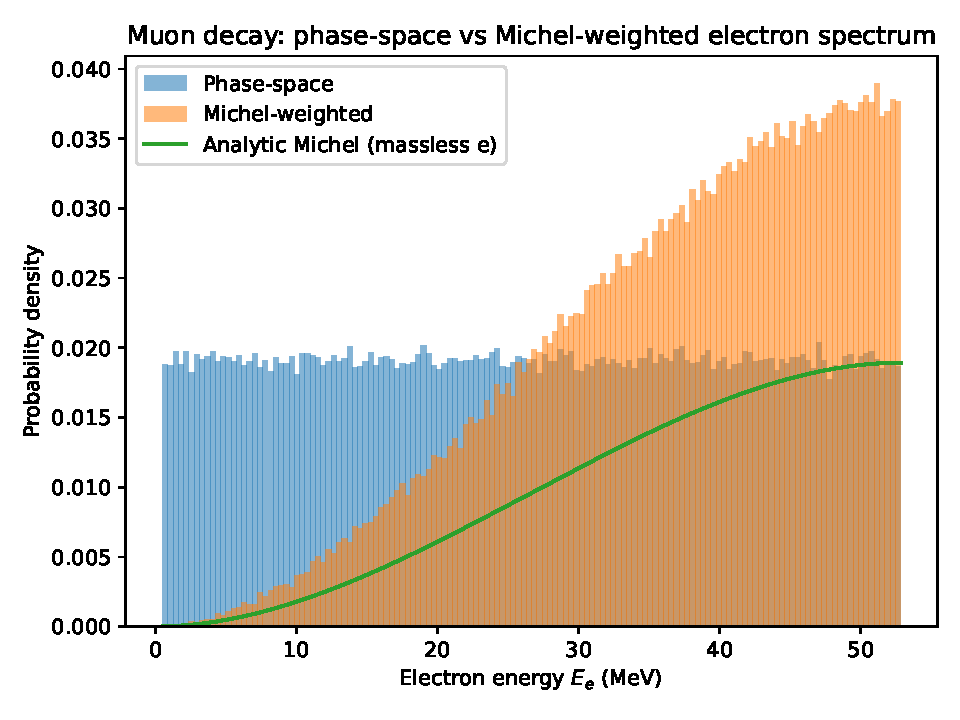
\includegraphics[width=\linewidth]{figures/fig_muon_michel_spectrum.pdf}
    \caption{Electron energy spectrum.}
    \label{fig:muon_michel}
  \end{subfigure}
  \hfill
  \begin{subfigure}[t]{0.49\linewidth}
    \centering
    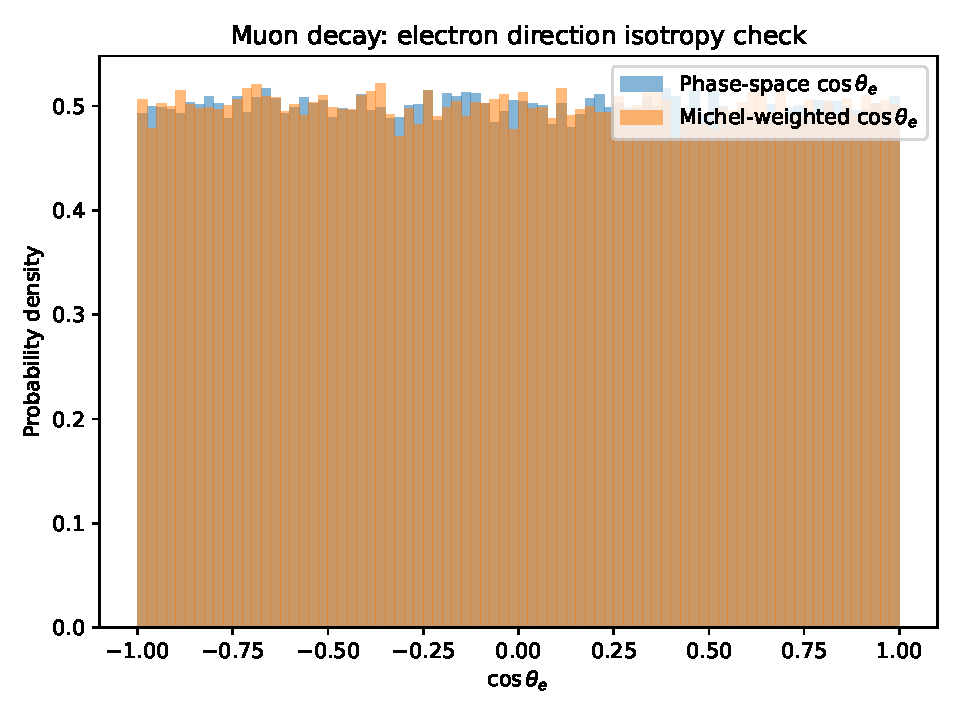
\includegraphics[width=\linewidth]{figures/fig_muon_cos_theta.pdf}
    \caption{Isotropy check using $\cos\theta_e$.}
    \label{fig:muon_costheta}
  \end{subfigure}
  \caption{Muon decay validation in the muon rest frame: electron spectrum shaping by
  Michel weighting, and isotropy of emission.}
  \label{fig:muon_distributions}
\end{figure}
\FloatBarrier

\paragraph{Event level conservation residuals.}
Energy and momentum conservation are enforced by construction. As an implementation check,
the residual
\begin{equation}
\Delta P^\mu = P_{\text{parent}}^\mu - \sum_i P_i^\mu
\end{equation}
is computed event by event. Figure \ref{fig:muon_conservation} shows the distributions of
$|\Delta E|$ and $|\Delta \p|$. Residuals concentrated near numerical precision indicate
consistent kinematic construction and transformations.

\begin{figure}[ht]
  \centering
  \begin{subfigure}[t]{0.49\linewidth}
    \centering
    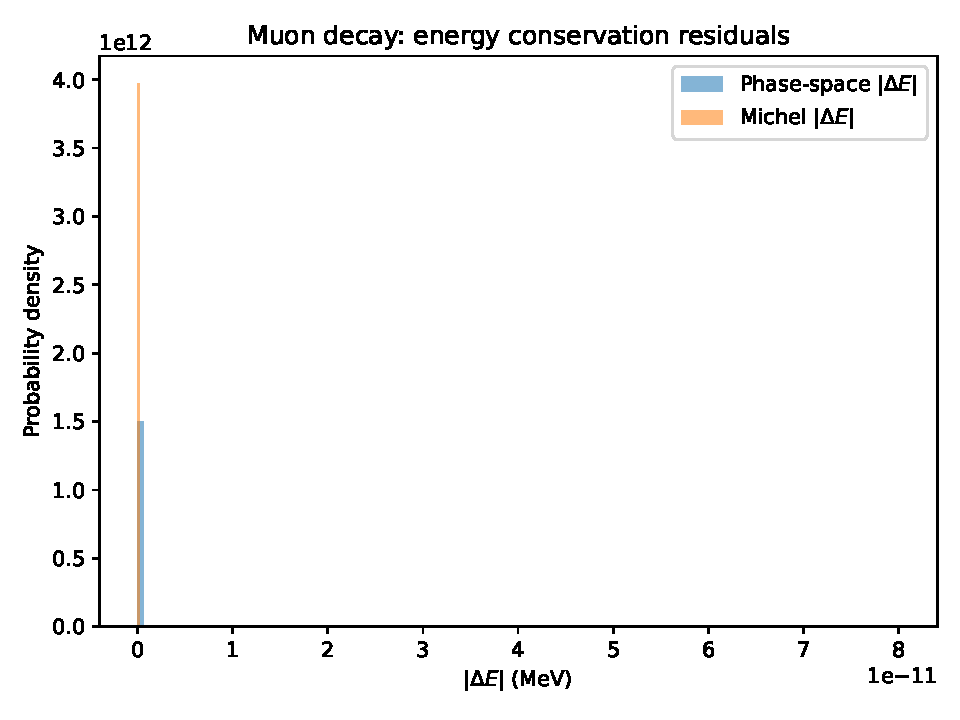
\includegraphics[width=\linewidth]{figures/fig_muon_conservation_deltaE.pdf}
    \caption{Energy residual $|\Delta E|$.}
    \label{fig:muon_deltaE}
  \end{subfigure}
  \hfill
  \begin{subfigure}[t]{0.49\linewidth}
    \centering
    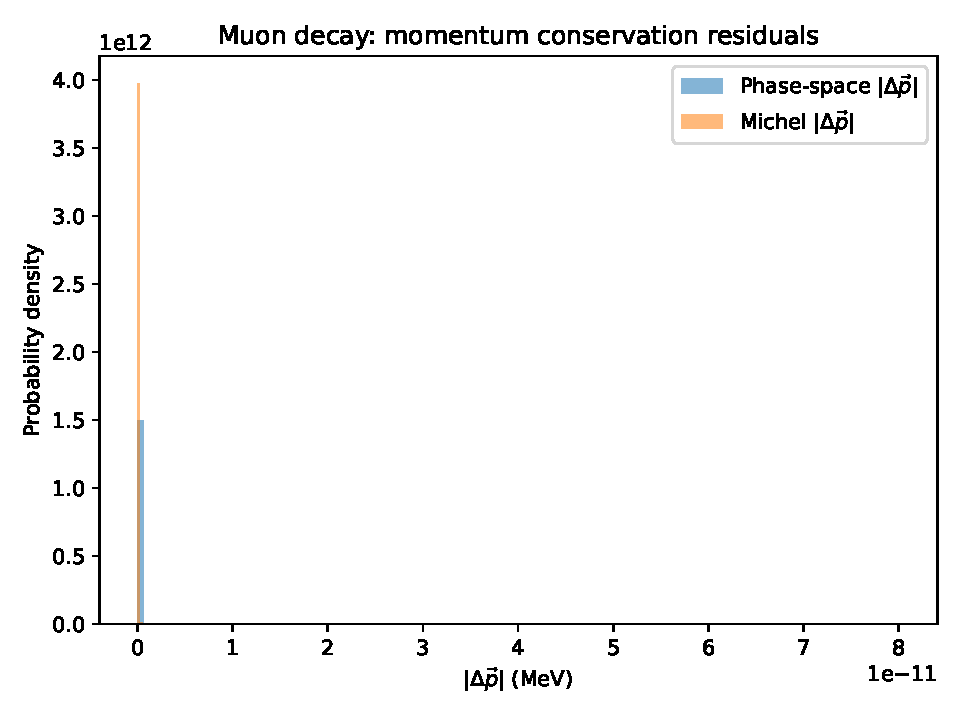
\includegraphics[width=\linewidth]{figures/fig_muon_conservation_deltaP.pdf}
    \caption{Momentum residual $|\Delta \p|$.}
    \label{fig:muon_deltaP}
  \end{subfigure}
  \caption{Muon decay conservation residuals for phase space and Michel weighted samples.}
  \label{fig:muon_conservation}
\end{figure}
\FloatBarrier

\subsection{Rutherford scattering validation}

Rutherford scattering is used to test numerical integration of sharply peaked angular
distributions and the effectiveness of importance sampling.

\paragraph{Differential cross section shape.}
Figure \ref{fig:rutherford_dsdomega} shows the angular dependence of the implemented
Rutherford form within the acceptance region. The strong forward enhancement motivates
angular regularization and informed sampling strategies.

\begin{figure}[ht]
  \centering
  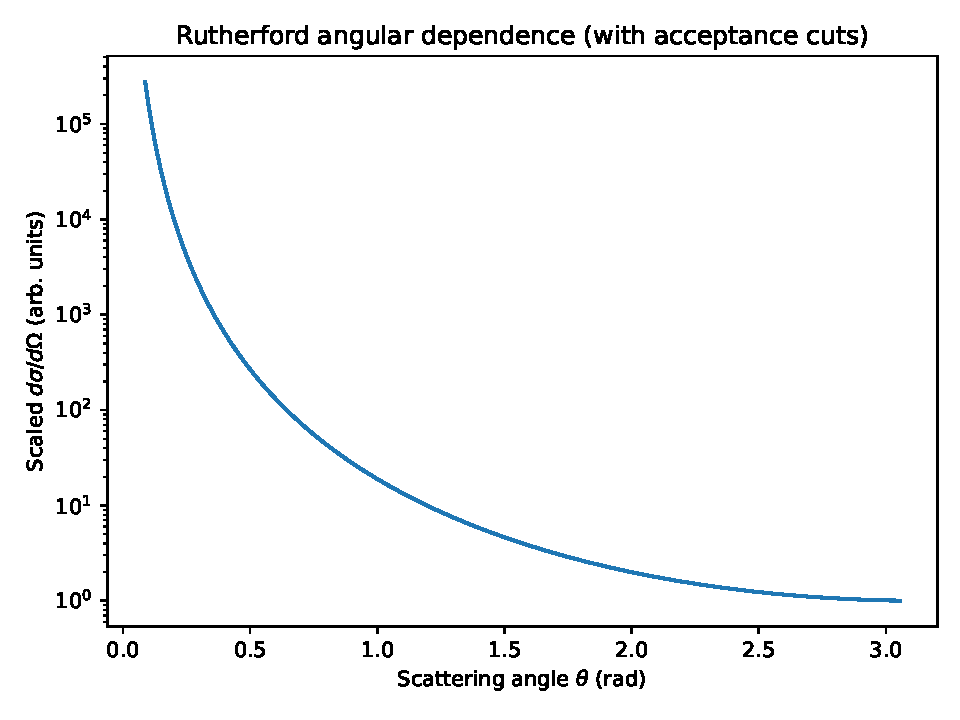
\includegraphics[width=0.85\linewidth]{figures/fig_rutherford_dsdomega.pdf}
  \caption{Rutherford angular dependence within the applied acceptance cuts.}
  \label{fig:rutherford_dsdomega}
\end{figure}
\FloatBarrier

\paragraph{Monte Carlo convergence of the total cross section.}
With acceptance cuts, the total cross section becomes finite and can be estimated by Monte
Carlo integration. A quadrature estimate provides a benchmark. Figure
\ref{fig:rutherford_sigma_conv} shows the Monte Carlo estimate as a function of sample
count alongside the quadrature value.

\begin{figure}[ht]
  \centering
  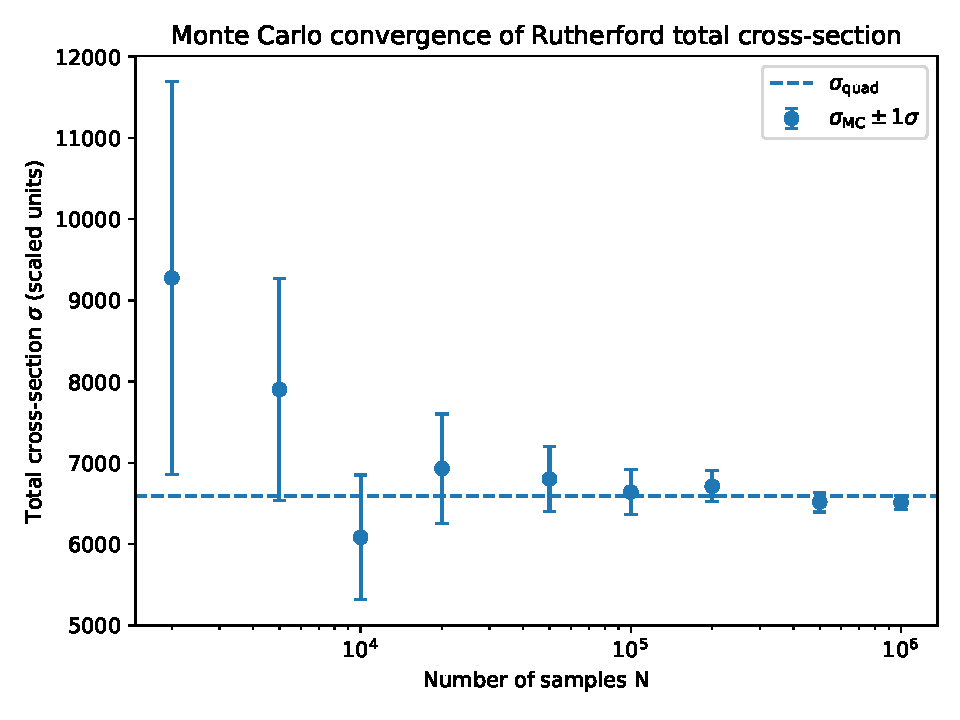
\includegraphics[width=0.85\linewidth]{figures/fig_rutherford_sigma_convergence.pdf}
  \caption{Convergence of the Monte Carlo estimate of the Rutherford total cross section.}
  \label{fig:rutherford_sigma_conv}
\end{figure}
\FloatBarrier

\paragraph{Validation of $\theta$ sampling.}
For importance sampling, the sampled $\theta$ distribution should match the normalized target
density proportional to $(d\sigma/d\Omega)\sin\theta$ over the accepted region. Figure
\ref{fig:rutherford_theta_pdf} compares the sampled histogram to this target density.

\begin{figure}[ht]
  \centering
  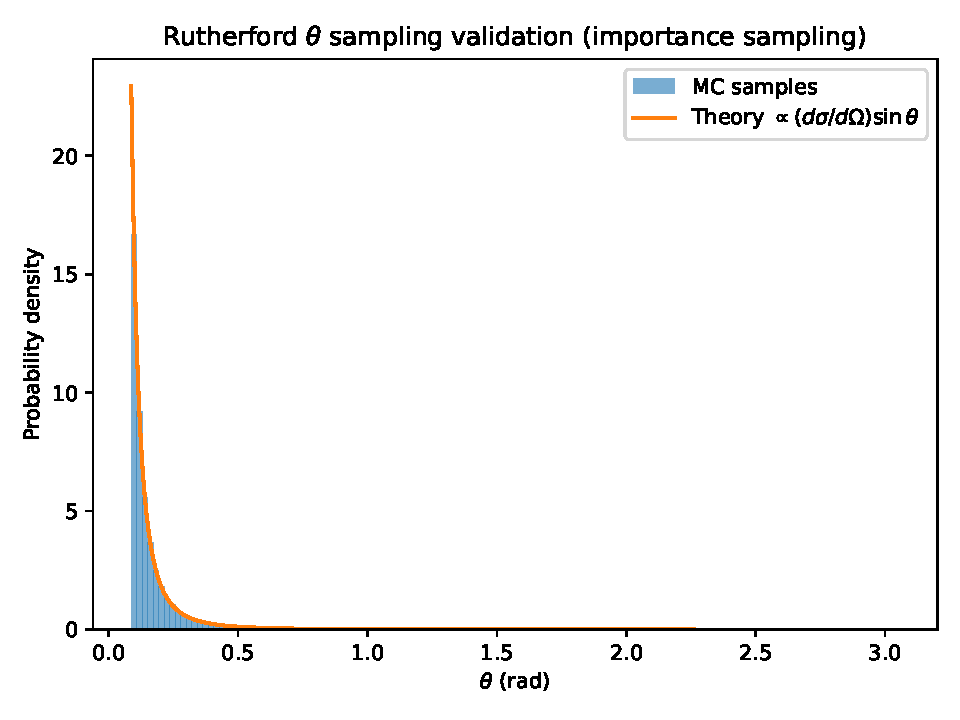
\includegraphics[width=0.85\linewidth]{figures/fig_rutherford_theta_pdf.pdf}
  \caption{Validation of Rutherford $\theta$ importance sampling against the target density.}
  \label{fig:rutherford_theta_pdf}
\end{figure}
\FloatBarrier

\subsection{Reproducibility artifacts}

The figure scripts also produce compact data products that allow inspection of the validation
checks without rerunning long jobs. The main artifacts are:
\begin{itemize}
  \item \texttt{muon\_spectra.npz}, containing electron energies, angular samples, and conservation residuals.
  \item \texttt{rutherford\_sigma\_convergence.csv}, containing the convergence table and benchmark values.
  \item \texttt{rutherford\_theta\_samples.npz}, containing sampled angles and target density information.
\end{itemize}


% =========================================================
\section{Software Structure and Reproducibility}
\label{sec:software}

The \texttt{decaymc} package is designed to be small, readable, and reproducible. The
implementation favors explicit physics logic and validation over performance oriented
optimization.

\subsection{Repository structure}

The repository is organized as follows:
\begin{itemize}
  \item \texttt{src/decaymc/}: core package source code, including kinematics, sampling,
  decay generators, and scattering utilities.
  \item \texttt{tests/}: unit tests covering kinematic identities, decay event generation,
  and scattering estimators.
  \item \texttt{scripts/}: small executable scripts, including a smoke test and figure
  generation scripts.
  \item \texttt{pyproject.toml}: package metadata and build configuration.
  \item \texttt{CITATION.cff}: citation metadata for software use and attribution.
\end{itemize}

\subsection{Installation}

The package can be installed in editable mode from the repository root:
\begin{equation}
\texttt{pip install -e .}
\end{equation}
This installs the package and its runtime dependencies. Development dependencies include
\texttt{pytest} for running the test suite.

\subsection{Running tests}

Correctness is supported by automated tests. From the repository root, the test suite can
be executed with:
\begin{equation}
\texttt{pytest -q}
\end{equation}
These tests check conservation laws, kinematic identities, and expected numerical behavior
of selected estimators.

\subsection{Reproducing figures}

All figures used in this report are generated by scripts included in the repository. The
figure scripts read and write local data products in standard formats (such as \texttt{.npz}
and \texttt{.csv}) so that intermediate results can be inspected without rerunning full
simulations.

A typical workflow is:
\begin{itemize}
  \item generate or load the required data products,
  \item produce plots from those data products,
  \item store both plots and the underlying numeric outputs for inspection and reuse.
\end{itemize}

\subsection{Versioning and citation}

The repository uses semantic versioning and tags releases. If the package is used in
downstream work, the recommended citation information is provided in \texttt{CITATION.cff}.


% =========================================================
\section{Limitations and Future Extensions}
\label{sec:limitations}

The scope of \texttt{decaymc} is intentionally narrow. The package is designed as a
transparent reference implementation for relativistic kinematics and Monte Carlo sampling,
not as a complete phenomenological event generator. The following limitations apply.

\subsection{Limitations}

\begin{itemize}
  \item Spin and polarization effects are not modeled, except insofar as they appear
  implicitly through the unpolarized Michel energy spectrum used in muon decay weighting.
  \item Radiative corrections and higher order effects are not included.
  \item Neutrinos are treated as massless, and other small mass effects are neglected where
  they do not affect the intended validation checks.
  \item No detector effects are included, such as resolution smearing, acceptance modeling,
  trigger effects, or reconstruction.
  \item The Rutherford scattering model is used as a controlled test case with explicit
  angular acceptance cuts. It should not be interpreted as a realistic description of
  screened Coulomb scattering in matter.
  \item The implementation prioritizes clarity over performance and is not intended for
  high throughput event generation.
\end{itemize}

\subsection{Future extensions}

The current structure makes several extensions straightforward if additional realism or
capabilities are desired:
\begin{itemize}
  \item Lorentz transforming generated decays to boosted laboratory frames and validating
  boosted frame distributions.
  \item Adding optional spin and polarization handling in a controlled way for selected
  processes.
  \item Implementing alternative three body phase space samplers and comparing efficiency
  and distribution quality.
  \item Extending scattering examples to include additional differential cross sections and
  comparing sampling strategies.
  \item Improving packaging and documentation for wider reuse while preserving the
  transparency of the core implementation.
\end{itemize}

These extensions are intentionally left outside the present scope so that the current
implementation remains compact and its validation remains unambiguous.


% =========================================================
\section{Conclusion}
\label{sec:conclusion}

This report has presented a transparent Monte Carlo implementation of relativistic
particle decays and scattering, with an emphasis on physical clarity and systematic
verification. Standard two body and three body decay kinematics were constructed from
first principles, and their numerical implementation was validated using conservation
laws, isotropy checks, known analytic distributions, and Monte Carlo convergence studies.

Three body decays were generated using a factorized construction based on an intermediate
system, which makes kinematic constraints explicit and provides a flexible proposal
distribution for additional weighting. This approach was used to implement muon decay,
where accept reject weighting reproduces the Michel electron energy spectrum while
maintaining exact energy and momentum conservation at the event level.

Rutherford scattering was used as a controlled example of Monte Carlo integration in the
presence of a sharply peaked differential cross section. The use of explicit angular
regularization and importance sampling illustrates how numerical efficiency and estimator
stability can be improved without obscuring the underlying physics.

The accompanying \texttt{decaymc} codebase is intentionally compact and favors explicit
logic over performance oriented optimization. It is intended as a reference
implementation that links relativistic kinematics, Monte Carlo sampling strategies, and
numerical validation in a reproducible way.

Overall, this work demonstrates that a small and carefully structured Monte Carlo framework
can serve as an effective tool for understanding and validating relativistic decay and
scattering processes, and can provide a solid foundation for further methodological or
educational extensions.


\bibliographystyle{unsrt}
\bibliography{references}

\end{document}

